\documentclass[12pt, addpoints]{exam/exam}

\usepackage{hyperref}
%\usepackage{mdframed}
\usepackage{graphicx, caption}	
%\usepackage{array, multicol, tabu}
\usepackage{amsmath, amsthm, amssymb}
\usepackage{comment}
\usepackage{enumitem}
\usepackage{url}
\usepackage{textcomp}
\newcommand{\1}{^{-1}}
\newcommand{\vect}[1]{\mathbf{#1}}
\newcommand{\R}{\mathbb R}
\newcommand{\vstr}{\vspace{\stretch{1}}}
\everymath{\displaystyle}
\setlength{\parindent}{0pt}

\theoremstyle{plain}
\newtheorem{thm}{Theorem}
\newtheorem*{thm*}{Theorem}

\DeclareMathOperator{\arcsec}{arcsec}

%\printanswers
\pointformat{\bf(\thepoints)}
\pointpoints{pt}{pts}
\bonuspointformat{\bf(\thepoints)}
\bonuspointpoints{pt}{pts}

\coverfirstpageheader{\bf MATH 236 (Calculus II) \\
		Fall 2017 \\
		}
		{}
		{{Name:} \underline{\hspace{40ex}} \\
		\vspace{0.5pc}
		Thur 28 Sep 2017}
\coverextraheadheight[2pc]{0in}
\coverfirstpagefooter{}{}{\Large Good luck!}
\coverrunningheader{}
	{Exam 1: Integrals}
	{}
\coverrunningheadrule	
\coverrunningfootrule
\coverrunningfooter{Wheeler}{Calc II Fall 2017}{p. \thepage\ (of \numpages)}

\firstpageheader{}
	{Exam 1: Integrals}
	{}
\firstpageheadrule
\firstpagefootrule
\firstpagefooter{Wheeler}{Calc II Fall 2017}{p. \thepage\ (of \numpages)}

\runningheadrule
\runningheader{}
	{Exam 1: Integrals}
	{}
\runningfootrule
\runningfooter{Wheeler}{Calc II Fall 2017}{p. \thepage\ (of \numpages)}

\title{\vspace{-8pc}
\vfill{\Huge
	\bf Exam 1: Integrals (\S4.5, 4.7, 5.1-5.5, 6.1-6.2, 6.4)} 
	}
%\author{}
\date{}

% % % % % % % % % % % % % % % % % % % %
\begin{document}

\begin{coverpages}
\maketitle
\thispagestyle{headandfoot}
\vspace{-4pc}
{\bf Exam Instructions:} You have 75 minutes to complete this exam.  Justification is required for all problems.  Notation matters!  You will also be penalized for missing units and rounding errors.  

\vspace{1pc}
No electronic devices (phones, iDevices, computers, etc) except for a \textbf{basic scientific calculator}.  On story problems, round to one decimal place. If you don't have a calculator, write ``no calculator" and simplify as far as you can.

\vspace{1pc}
If you finish early then you may leave, UNLESS there are less than 5 minutes of class left.  To prevent disruption, if you finish with less than 5 minutes of class remaining then please stay seated and quiet.

\begin{flushright}
%In addition, please provide the following data:

\vspace{0.3in}
%Drill Instructor: \underline{\hspace{40ex}}

\vspace{0.3in}
%Drill Time: \underline{\hspace{40ex}}
\end{flushright}

\vfill
\textbf{Your signature below indicates that you have read this page and agree to follow the Academic Honesty Policies of James Madison University.}  

\vspace{0.3in}
Signature: {\bf (1 pt)} \underline{\hspace{73ex}}

% % % % % % % % % %
\newpage
\textbf{Formulas you may need:}

\vspace{1pc}
$\frac{d}{dx}\arcsin x=\frac{1}{\sqrt{1-x^2}}$; domain of $\arcsin x$: $[-1,1]$; range of $\arcsin x$: $[-\frac{\pi}{2},\frac{\pi}{2}]$

$\frac{d}{dx}\arctan x=\frac{1}{x^2+1}$; domain of $\arctan x$: $(-\infty, \infty)$; range of $\arctan x$: $(-\frac{\pi}{2},\frac{\pi}{2})$

$\frac{d}{dx}\arcsec x=\frac{1}{|x|\sqrt{x^2-1}}$; domain of $\arcsec x$: $(-\infty,-1]\cup [1,\infty)$; range of $\arcsec x$: $[0,\frac{\pi}{2}]\cup [\frac{\pi}{2},\pi]$

\vspace{1.5pc}
$\int \tan x\ dx=-\ln|\cos x|+C$

$\int \cot x\ dx=\ln|\sin x|+C$

$\int \sec x\ dx=\ln|\sec x\tan x|+C$

$\int \csc x\ dx=-\ln|\csc x\cot x|+C$

$\int \arcsin x\ dx=x\arcsin x+\sqrt{1-x^2}+C$

$\int \arctan x\ dx=x\arctan x-\frac{1}{2}\ln(x^2+1)+C$

\vspace{1.5pc}
$\sin^2x=\frac{1}{2}(1-\cos{2x})$

\vspace{0.25pc}
$\cos^2x=\frac{1}{2}(1+\cos{2x})$

\vspace{0.7pc}
$\sin{2x}=2\sin x\cos x$

\vfill
\gradetable 

\newpage
\textbf{Formulas, cont.}

\vspace{0.75pc}
mass = (density)(volume)

work = (force)(displacement)

hydrostatic force = (weight-density)(surface area)(depth of liquid)

weight-density of water = 62.4 lb/ft$^3$

\vspace{1.5pc}
\begin{tabular}{c | c | c}
Integral & Rewrite & Choose \\
\hline
$\int \sin^nx\ dx$, $n$ odd & $\int\text{(expression in $\cos x$)}\sin x$ & $u=\cos x$ \\
\hline
$\int \sin^mx\cos^nx\ dx$, $n$ odd & $\int\text{(expression in $\sin x$)}\cos x$ & $u=\sin x$ \\
\hline
$\int \sin^mx\cos^nx\ dx$, $m$ odd & $\int\text{(expression in $\cos x$)}\sin x$ & $u=\cos x$ \\
\hline
$\int \sec^mx\tan^nx\ dx$, $m$ even & $\int\text{(expression in $\tan x$)}\sec^2 x$ & $u=\tan x$ \\
\hline
$\int \sec^mx\tan^nx\ dx$, $n$ odd & $\int\text{(expression in $\sec x$)}\sec x\tan x$ & $u=\sec x$
\end{tabular}

\vspace{1.5pc}
$(A+B)^n=\sum_{k=0}^n \frac{n!}{k!(n-k)!}A^kB^{n-k}$

\end{coverpages}

% % % % % % % % % % % % % % % % % % % %
\begin{questions}
\thispagestyle{headandfoot}

% % % % %
\question Compute the following derivatives.
	\begin{parts}
	\part[9] %{\bf \S4.7 \#44} 
	$\displaystyle \frac{d^2}{dx^2}\int_1^{e^x}f(t)g(t)\ dt$
	\vspace{22pc}
	
	\part[9] %{\bf \S4.7 \#46} 
	$\displaystyle \frac{d}{dx}\left(x^2\int_0^{\sin x}\sqrt t\ dt \right)$
	\vspace{22pc}
	\end{parts}

\newpage
% % % % % 
\question[20] %{\bf \S5.3 \#48} 
Evaluate: $\displaystyle \int_{-1}^1\frac{4(x^2-1)}{x^2-4}\ dx$ 

\newpage
% % % % %
\question[25] %{\bf \S5.5 \#72} 
Evaluate: $\displaystyle \int e^{2x}(1-e^{4x})^{\frac{3}{2}}\ dx$

\newpage
% % % % %
\question[18] %{\bf \S6.2 \#58} 
Find the volume of the solid of revolution given by the region bounded by the graphs of $f(x)=2\ln x$, $y=0$, $y=3$, and $x=0$, revolved around the $x$-axis.
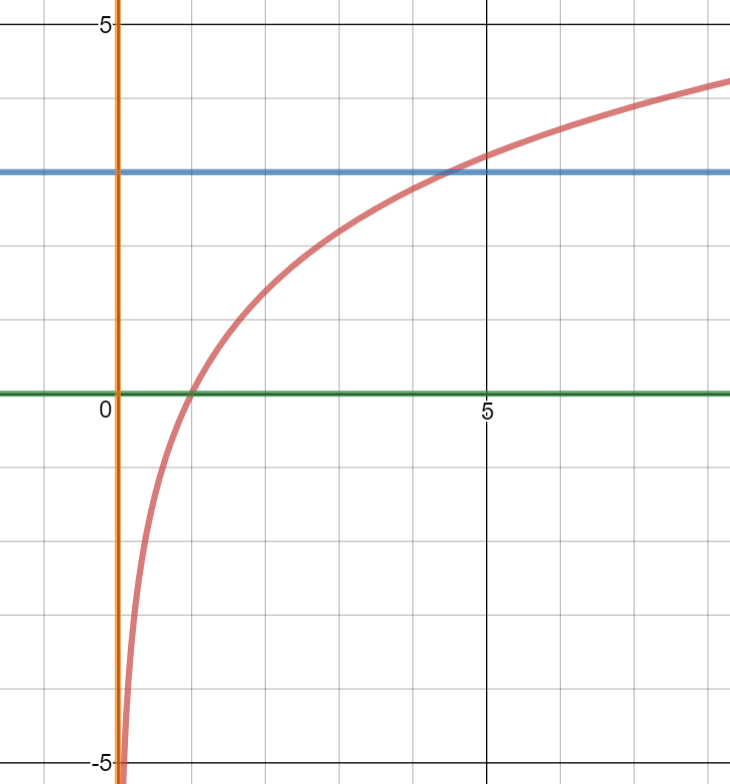
\includegraphics[scale=0.4]{Calc2Exam16-2_58.png}

\newpage
% % % % %
\question[18] %{\bf \S6.4 \# 56} 
Find the work required to pump all the liquid out of the top of a tank and up to 4 feet above ground level, given that the tank is a giant upright cylinder with a radius of 8 feet and a height of 20 feet, buried so that its top is 2 feet below the surface.  The tank is only two-thirds full and contains a strange liquid that weighs 71.8 pounds per cubic foot.

\end{questions}

\end{document}